\documentclass{letter}
\usepackage[margin=0.75in]{geometry}
\usepackage{amsmath}
\usepackage{amssymb}
\usepackage{enumerate}
\usepackage{changepage}
\usepackage{tikz}
\usepackage{pgfplots}
\usetikzlibrary{arrows}
\pgfplotsset{compat=1.8}
\def\myrad{2cm}
\def\myang{30}
\pgfplotsset{vasymptote/.style={
		before end axis/.append code={
			\draw[densely dashed] ({rel axis cs:0,0} -| {axis cs:#1,0})
			-- ({rel axis cs:0,1} -| {axis cs:#1,0});
		}
	}}

\begin{document}
	\begin{center}
		\LARGE Math135 - November 16, 2015\\
		\large Complex Modulus - Polar Coordinates
	\end{center}
	\vspace{0.25 in}
	\underline{\textbf{Complex Modulus}}
	
	The modulus of the complex number $z = x + yi$ is the non-negative real number:
	
	\[ \mid z \mid\; = \;\mid x + yi \mid\; = \sqrt{x^2 + y^2} \]
	
	We cannot order complex numbers, but using the modulus gives us a way to compare them.
	
	\begin{itemize}
		\item[Ex. ] If $z = 3 - 5i$, then\\
		$\vert z \vert = \sqrt{3^2 + (-5)^2}$\\
		$\vert z \vert = \sqrt{34}$
	\end{itemize}
	
	\underline{\textbf{Properties of Modulus}}
	
	If $z$ and $w$ are complex numbers, then
	\begin{enumerate}[1.]
		\item $\vert z \vert = 0$ if and only if$z=0$
		\item $\vert \overline{z} \vert = \vert z \vert$
		\item $\overline{z} z = \vert z \vert ^2$
		\item $\vert z w \vert = \vert z \vert \vert w \vert$
		\item $\vert z + w\vert \leq \vert z \vert + \vert w \vert$
	\end{enumerate}
	
	\begin{itemize}
		\item[Ex. ] Let $z \in \mathbb{C}$ such that $z \neq \pm i$\\
		Prove $\dfrac{z}{1+x^2} \in \mathbb{R} \iff z \in \mathbb{R}$ or $\vert z \vert = 1$
		
		Assume $\dfrac{z}{1+z^2} \in \mathbb{R}$.
		
		\begin{flalign*}
			\dfrac{z}{1+z^2} &= \overline{\dfrac{z}{1+z^2}}&\\
			&= \dfrac{\overline{z}}{1+ (\overline{z})^2}\\
			z(1+\overline{z}^2) &= \overline{z}(1+z^2)\\
			z + z\overline{z}^2 &= \overline{z} + \overline{z}z^2\\
			0 &= z - \overline{z} + z\overline{z}^2 - \overline{z}z^2\\
		&= z - \overline{z} - z\overline{z}(\overline{z} + z)\\
		&= (z - \overline{z})(1- z\overline{z})
		\end{flalign*}
		
		So, $z = z\overline{z} \in \mathbb{R}$ or $\vert z \vert = 1$
		Since all steps taken in this proof are reversible, we don't have to prove the iff the other way.
	\end{itemize}
	\clearpage
	\underline{\textbf{The Complex Plane}}
	
		\textbf{Ex. } Graph $-2 + 3i$.\\
			\begin{tikzpicture}
			\coordinate (a) at (6,3);
			\coordinate (b) at (2,4);
			\begin{axis}[
			x label style={at={(axis description cs:0.5,-0.1)},anchor=north},
			y label style={at={(axis description cs:-0.1,.5)},rotate=90,anchor=south},
			xlabel={Re},
			ylabel={\;\;Im},
			axis equal image,
			axis lines=middle,
			xmin=-5,xmax=5,
			ymin=0,ymax=5,
			enlargelimits={abs=1cm},
			axis line style={latex-latex},
			yticklabel style={anchor=west},
			ytick={},
			xtick={},
			vasymptote=0,
			]
			% This doesn't clip to y=-10:10 nicely
			% because there are too few samples near the asymptote:
			
			\addplot[dashed, black, domain=-2:0,samples=200, restrict y to domain=0:100]
			{((-3/2)*(x)};
			\addplot[only marks] table {
				-2 3
			};
			\end{axis}
			\end{tikzpicture}
			
			This is called an Argand Diagram.
			
			Thinking graphically, the \textbf{conjugate} is a reflection in the real axis.\\
			The \textbf{modulo} is the distance from the origin (0,0).\\
			\textbf{Addition} is like vector addition. You draw the line from the origin to one point, draw a line from the origin to the other point, then append one line on the end of the other line to 
			
			\underline{\textbf{Polar Coordinates}}
			
			Polar coordinates offer a way to think of complex numbers in terms of a magnitude and an angle. To construct a polar coordinate, imagine the magnitude $r$ as a point on the positive real axis. Then, rotate this point $\theta$ radians around a circle centered at the origin with a radius $r$. When working with polar coordinates, the origin is called the \textbf{pole}, and the positive real axis is called the \textbf{polar axis}.
			
			\begin{center}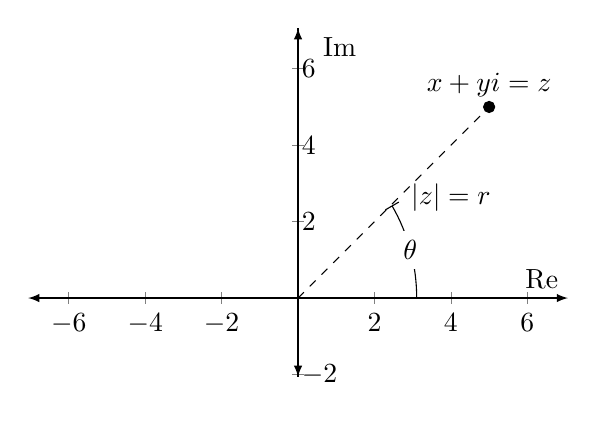
\begin{tikzpicture}
				\coordinate (a) at (6,3);
				\coordinate (b) at (2,4);
				\begin{axis}[
				x label style={at={(axis description cs:0.5,-0.1)},anchor=north},
				y label style={at={(axis description cs:-0.1,.5)},rotate=90,anchor=south},
				xlabel={Re},
				ylabel={\;\;Im},
				axis equal image,
				axis lines=middle,
				xmin=-5,xmax=5,
				ymin=0,ymax=5,
				enlargelimits={abs=1cm},
				axis line style={latex-latex},
				yticklabel style={anchor=west},
				ytick={},
				xtick={},
				vasymptote=0,
				]
				\node [above] at (axis cs:  5, 5) {$x + yi = z$};
				\node [above] at (axis cs:  4, 2) {$\vert z \vert = r$};
				\draw[|-|]
				(\myrad+55pt,0)
				arc[start angle=0,end angle=\myang,radius=\myrad+10pt]
				node[midway,fill=white] {$\theta$};
				\addplot[dashed, black, domain=0:5,samples=200, restrict y to domain=0:100]
				{((1)*(x)};
				\addplot[only marks] table {
					5 5
				};
				\end{axis}
				\end{tikzpicture}\end{center}
			
			$r = \vert x \vert = \sqrt{x^2 + y^2}$\\
			$\theta = $the counter-clockwise angle of rotation from the polar axis measured in radians.\\
			$(r, \theta)$ represents a number in the complex number system. Using this notation, every number can be represented an infinite number of ways, because:
			
			$(r, \theta) = (r, \theta + 2k \pi), k \in \mathbb{Z}$
\end{document}